\documentclass[a4paper]{book}
\usepackage{a4wide}
\usepackage{makeidx}
\usepackage{graphicx}
\usepackage{multicol}
\usepackage{float}
\usepackage{listings}
\usepackage{color}
\usepackage{textcomp}
\usepackage{alltt}
\usepackage{times}
\usepackage{ifpdf}
\ifpdf
\usepackage[pdftex,
            pagebackref=true,
            colorlinks=true,
            linkcolor=blue,
            unicode
           ]{hyperref}
\else
\usepackage[ps2pdf,
            pagebackref=true,
            colorlinks=true,
            linkcolor=blue,
            unicode
           ]{hyperref}
\usepackage{pspicture}
\fi
\usepackage[utf8]{inputenc}
\usepackage{doxygen}
\lstset{language=C++,inputencoding=utf8,basicstyle=\footnotesize,breaklines=true,breakatwhitespace=true,tabsize=8,numbers=left }
\makeindex
\setcounter{tocdepth}{3}
\renewcommand{\footrulewidth}{0.4pt}
\begin{document}
\hypersetup{pageanchor=false}
\begin{titlepage}
\vspace*{7cm}
\begin{center}
{\Large pokerTemplate }\\
\vspace*{1cm}
{\large Generated by Doxygen 1.6.3}\\
\vspace*{0.5cm}
{\small Sat Feb 19 10:20:55 2011}\\
\end{center}
\end{titlepage}
\clearemptydoublepage
\pagenumbering{roman}
\tableofcontents
\clearemptydoublepage
\pagenumbering{arabic}
\hypersetup{pageanchor=true}
\chapter{Class Index}
\section{Class Hierarchy}
This inheritance list is sorted roughly, but not completely, alphabetically:\begin{DoxyCompactList}
\item \contentsline{section}{MessageBox}{\pageref{d2/da3/classMessageBox}}{}
\item \contentsline{section}{SettingManager}{\pageref{d5/df2/classSettingManager}}{}
\item \contentsline{section}{Thread$<$ TM $>$}{\pageref{d6/d40/classThread_3_01TM_01_4}}{}
\item \contentsline{section}{ThreadManager}{\pageref{de/d57/classThreadManager}}{}
\begin{DoxyCompactList}
\item \contentsline{section}{Engine}{\pageref{d1/db6/classEngine}}{}
\item \contentsline{section}{Module}{\pageref{d3/d9c/classModule}}{}
\end{DoxyCompactList}
\end{DoxyCompactList}

\chapter{Class Index}
\section{Class List}
Here are the classes, structs, unions and interfaces with brief descriptions:\begin{DoxyCompactList}
\item\contentsline{section}{\hyperlink{classEngine}{Engine} }{\pageref{d1/db6/classEngine}}{}
\item\contentsline{section}{\hyperlink{classMessageBox}{MessageBox} }{\pageref{d2/da3/classMessageBox}}{}
\item\contentsline{section}{\hyperlink{classModule}{Module} }{\pageref{d3/d9c/classModule}}{}
\item\contentsline{section}{\hyperlink{classSettingManager}{SettingManager} }{\pageref{d5/df2/classSettingManager}}{}
\item\contentsline{section}{\hyperlink{classThread_3_01TM_01_4}{Thread$<$ TM $>$} }{\pageref{d6/d40/classThread_3_01TM_01_4}}{}
\item\contentsline{section}{\hyperlink{classThreadManager}{ThreadManager} }{\pageref{de/d57/classThreadManager}}{}
\end{DoxyCompactList}

\chapter{Class Documentation}
\hypertarget{classEngine}{
\section{Engine Class Reference}
\label{d1/db6/classEngine}\index{Engine@{Engine}}
}


{\ttfamily \#include $<$engine.h$>$}

Inheritance diagram for Engine:\begin{figure}[H]
\begin{center}
\leavevmode
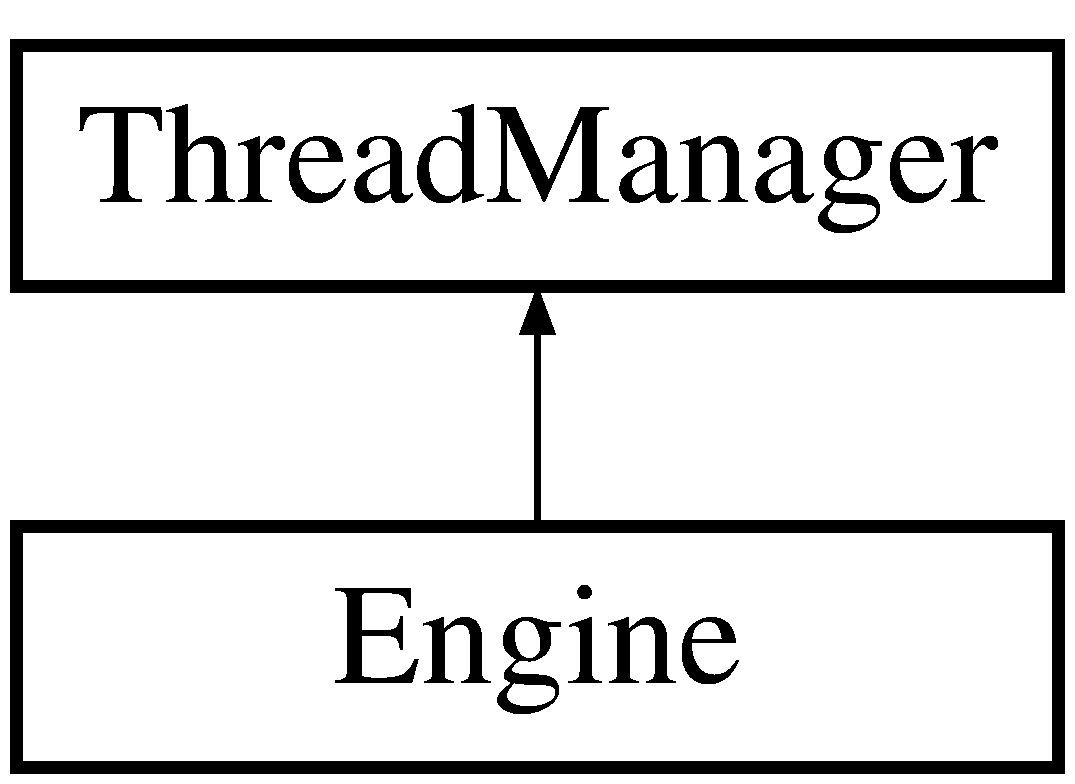
\includegraphics[height=2cm]{d1/db6/classEngine}
\end{center}
\end{figure}
\subsection*{Public Member Functions}
\begin{DoxyCompactItemize}
\item 
virtual void \hyperlink{classEngine_a5de6694a069170d2205599331e6e8691}{Create} (boost::shared\_\-ptr$<$ Thread $>$ thread)
\item 
virtual void \hyperlink{classEngine_afe5c1c859cfe9b121627156dfbd58e6b}{Join} (int index)
\item 
\hypertarget{classEngine_ade901a4373d3ee77b6eb716ce84dc9bb}{
virtual void {\bfseries Destroy} ()}
\label{d1/db6/classEngine_ade901a4373d3ee77b6eb716ce84dc9bb}

\item 
\hyperlink{classEngine_a8c98683b0a3aa28d8ab72a8bcd0d52f2}{Engine} ()
\item 
\hyperlink{classEngine_a8ef7030a089ecb30bbfcb9e43094717a}{$\sim$Engine} ()
\end{DoxyCompactItemize}


\subsection{Detailed Description}
\begin{DoxyAuthor}{Author}
Kevin TRAN 
\end{DoxyAuthor}
\begin{DoxyVersion}{Version}
0.1 
\end{DoxyVersion}
\begin{DoxyDate}{Date}
16/02/2011 
\end{DoxyDate}
\hypertarget{d6/d40/classThread_3_01TM_01_4_LICENSE}{}\subsection{LICENSE}\label{d6/d40/classThread_3_01TM_01_4_LICENSE}
This file is part of \#PROJECT\#\#.

\#PROJECT\#\# is free software: you can redistribute it and/or modify it under the terms of the GNU General Public License as published by the Free Software Foundation, either version 3 of the License, or (at your option) any later version.

\#PROJECT\#\# is distributed in the hope that it will be useful, but WITHOUT ANY WARRANTY; without even the implied warranty of MERCHANTABILITY or FITNESS FOR A PARTICULAR PURPOSE. See the GNU General Public License for more details.

You should have received a copy of the GNU General Public License along with \#PROJECT\#\#. If not, see $<$\href{http://www.gnu.org/licenses/}{\tt http://www.gnu.org/licenses/}$>$.\hypertarget{d6/d40/classThread_3_01TM_01_4_DESCRIPTION}{}\subsection{DESCRIPTION}\label{d6/d40/classThread_3_01TM_01_4_DESCRIPTION}
Header for class \hyperlink{classEngine}{Engine}\hypertarget{d6/d40/classThread_3_01TM_01_4_HISTORY}{}\subsection{HISTORY}\label{d6/d40/classThread_3_01TM_01_4_HISTORY}
16/02/2011 : first draft 

\subsection{Constructor \& Destructor Documentation}
\hypertarget{classEngine_a8c98683b0a3aa28d8ab72a8bcd0d52f2}{
\index{Engine@{Engine}!Engine@{Engine}}
\index{Engine@{Engine}!Engine@{Engine}}
\subsubsection[{Engine}]{\setlength{\rightskip}{0pt plus 5cm}Engine::Engine ()}}
\label{d1/db6/classEngine_a8c98683b0a3aa28d8ab72a8bcd0d52f2}
default constructor \hypertarget{classEngine_a8ef7030a089ecb30bbfcb9e43094717a}{
\index{Engine@{Engine}!$\sim$Engine@{$\sim$Engine}}
\index{$\sim$Engine@{$\sim$Engine}!Engine@{Engine}}
\subsubsection[{$\sim$Engine}]{\setlength{\rightskip}{0pt plus 5cm}Engine::$\sim$Engine ()}}
\label{d1/db6/classEngine_a8ef7030a089ecb30bbfcb9e43094717a}
Destructor 

\subsection{Member Function Documentation}
\hypertarget{classEngine_a5de6694a069170d2205599331e6e8691}{
\index{Engine@{Engine}!Create@{Create}}
\index{Create@{Create}!Engine@{Engine}}
\subsubsection[{Create}]{\setlength{\rightskip}{0pt plus 5cm}virtual void Engine::Create (boost::shared\_\-ptr$<$ Thread $>$ {\em thread})\hspace{0.3cm}{\ttfamily  \mbox{[}virtual\mbox{]}}}}
\label{d1/db6/classEngine_a5de6694a069170d2205599331e6e8691}

\begin{DoxyParams}{Parameters}
\item[{\em thread}]\end{DoxyParams}


Implements \hyperlink{classThreadManager_afad6766592d98c6c0a2129f45e6a346e}{ThreadManager}.

\hypertarget{classEngine_afe5c1c859cfe9b121627156dfbd58e6b}{
\index{Engine@{Engine}!Join@{Join}}
\index{Join@{Join}!Engine@{Engine}}
\subsubsection[{Join}]{\setlength{\rightskip}{0pt plus 5cm}virtual void Engine::Join (int {\em index})\hspace{0.3cm}{\ttfamily  \mbox{[}virtual\mbox{]}}}}
\label{d1/db6/classEngine_afe5c1c859cfe9b121627156dfbd58e6b}

\begin{DoxyParams}{Parameters}
\item[{\em index}]\end{DoxyParams}


Implements \hyperlink{classThreadManager_a3c1b72b44ca4ffa3652088d44937b9d0}{ThreadManager}.



The documentation for this class was generated from the following file:\begin{DoxyCompactItemize}
\item 
src/core/engine.h\end{DoxyCompactItemize}

\hypertarget{classMessageBox}{
\section{MessageBox Class Reference}
\label{d2/da3/classMessageBox}\index{MessageBox@{MessageBox}}
}


{\ttfamily \#include $<$messageBox.h$>$}

\subsection*{Public Member Functions}
\begin{DoxyCompactItemize}
\item 
boost::shared\_\-pointer$<$ Message $>$ \hyperlink{classMessageBox_aea4614d2371b253e2e96f602bdd9c557}{ReadMessage} ()
\item 
void \hyperlink{classMessageBox_a26aab3fd74f9d025664448cef1fff9c0}{ReceiveMessage} (boost::shared\_\-pointer$<$ Message $>$ message)
\item 
\hyperlink{classMessageBox_adb0c3df8b7a04a515456f0f2bf47321b}{MessageBox} ()
\item 
\hyperlink{classMessageBox_a1db265f45271916de44a4f500ccc566d}{$\sim$MessageBox} ()
\end{DoxyCompactItemize}


\subsection{Detailed Description}
\begin{DoxyAuthor}{Author}
Kevin TRAN 
\end{DoxyAuthor}
\begin{DoxyVersion}{Version}
0.1 
\end{DoxyVersion}
\begin{DoxyDate}{Date}
14/02/2011 
\end{DoxyDate}
\hypertarget{d6/d40/classThread_3_01TM_01_4_LICENSE}{}\subsection{LICENSE}\label{d6/d40/classThread_3_01TM_01_4_LICENSE}
This file is part of \#PROJECT\#\#.

\#PROJECT\#\# is free software: you can redistribute it and/or modify it under the terms of the GNU General Public License as published by the Free Software Foundation, either version 3 of the License, or (at your option) any later version.

\#PROJECT\#\# is distributed in the hope that it will be useful, but WITHOUT ANY WARRANTY; without even the implied warranty of MERCHANTABILITY or FITNESS FOR A PARTICULAR PURPOSE. See the GNU General Public License for more details.

You should have received a copy of the GNU General Public License along with \#PROJECT\#\#. If not, see $<$\href{http://www.gnu.org/licenses/}{\tt http://www.gnu.org/licenses/}$>$.\hypertarget{d6/d40/classThread_3_01TM_01_4_DESCRIPTION}{}\subsection{DESCRIPTION}\label{d6/d40/classThread_3_01TM_01_4_DESCRIPTION}
Header for class \hyperlink{classMessageBox}{MessageBox}\hypertarget{d6/d40/classThread_3_01TM_01_4_HISTORY}{}\subsection{HISTORY}\label{d6/d40/classThread_3_01TM_01_4_HISTORY}
14/02/2011 : first draft 

\subsection{Constructor \& Destructor Documentation}
\hypertarget{classMessageBox_adb0c3df8b7a04a515456f0f2bf47321b}{
\index{MessageBox@{MessageBox}!MessageBox@{MessageBox}}
\index{MessageBox@{MessageBox}!MessageBox@{MessageBox}}
\subsubsection[{MessageBox}]{\setlength{\rightskip}{0pt plus 5cm}MessageBox::MessageBox ()}}
\label{d2/da3/classMessageBox_adb0c3df8b7a04a515456f0f2bf47321b}
default constructor \hypertarget{classMessageBox_a1db265f45271916de44a4f500ccc566d}{
\index{MessageBox@{MessageBox}!$\sim$MessageBox@{$\sim$MessageBox}}
\index{$\sim$MessageBox@{$\sim$MessageBox}!MessageBox@{MessageBox}}
\subsubsection[{$\sim$MessageBox}]{\setlength{\rightskip}{0pt plus 5cm}MessageBox::$\sim$MessageBox ()}}
\label{d2/da3/classMessageBox_a1db265f45271916de44a4f500ccc566d}
Destructor 

\subsection{Member Function Documentation}
\hypertarget{classMessageBox_aea4614d2371b253e2e96f602bdd9c557}{
\index{MessageBox@{MessageBox}!ReadMessage@{ReadMessage}}
\index{ReadMessage@{ReadMessage}!MessageBox@{MessageBox}}
\subsubsection[{ReadMessage}]{\setlength{\rightskip}{0pt plus 5cm}boost::shared\_\-pointer$<$Message$>$ MessageBox::ReadMessage ()}}
\label{d2/da3/classMessageBox_aea4614d2371b253e2e96f602bdd9c557}
Read oldest unread message received. Wait for it if there isn't any. \begin{DoxyReturn}{Returns}
read message 
\end{DoxyReturn}
\hypertarget{classMessageBox_a26aab3fd74f9d025664448cef1fff9c0}{
\index{MessageBox@{MessageBox}!ReceiveMessage@{ReceiveMessage}}
\index{ReceiveMessage@{ReceiveMessage}!MessageBox@{MessageBox}}
\subsubsection[{ReceiveMessage}]{\setlength{\rightskip}{0pt plus 5cm}void MessageBox::ReceiveMessage (boost::shared\_\-pointer$<$ Message $>$ {\em message})}}
\label{d2/da3/classMessageBox_a26aab3fd74f9d025664448cef1fff9c0}
Post a message to the message box. 
\begin{DoxyParams}{Parameters}
\item[{\em message}]the message to post. \end{DoxyParams}


The documentation for this class was generated from the following file:\begin{DoxyCompactItemize}
\item 
src/message/messageBox.h\end{DoxyCompactItemize}

\hypertarget{classModule}{
\section{Module Class Reference}
\label{d3/d9c/classModule}\index{Module@{Module}}
}


{\ttfamily \#include $<$module.h$>$}

Inheritance diagram for Module:\begin{figure}[H]
\begin{center}
\leavevmode
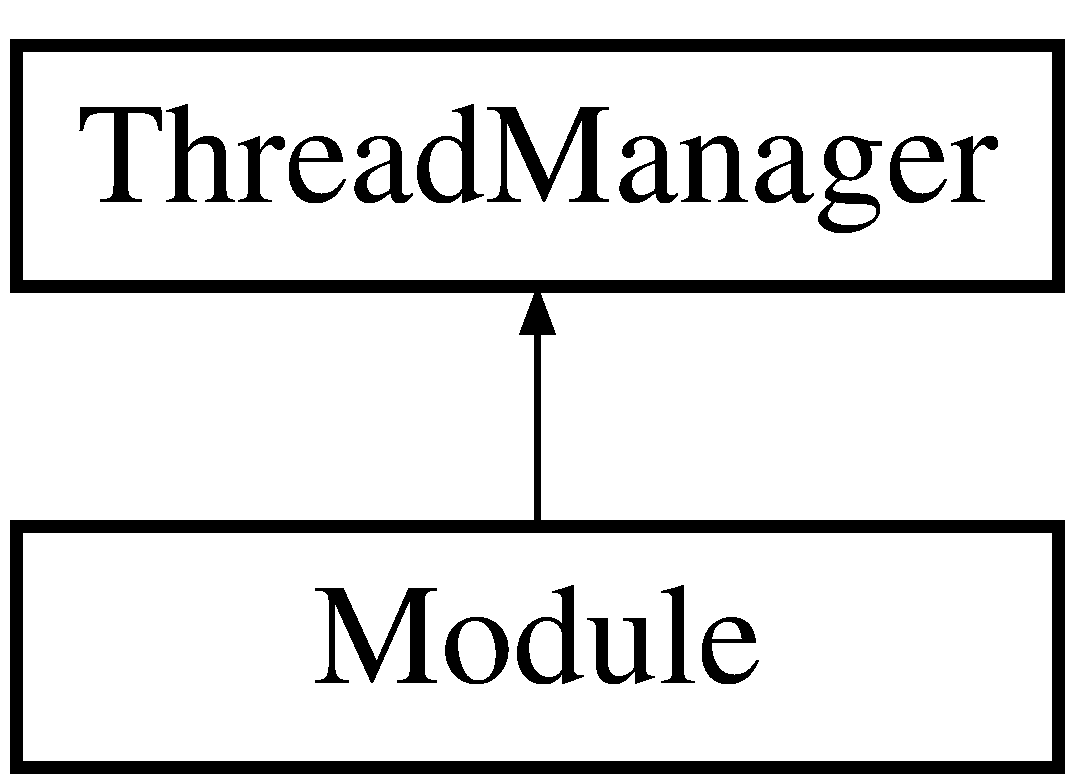
\includegraphics[height=2cm]{d3/d9c/classModule}
\end{center}
\end{figure}
\subsection*{Public Member Functions}
\begin{DoxyCompactItemize}
\item 
virtual void \hyperlink{classModule_a9984bf9d8b1ea6e280c8c47cdb56e906}{Create} (boost::shared\_\-ptr$<$ Thread $>$ thread)
\item 
virtual void \hyperlink{classModule_ac141815618543512136b7f4e0c90d311}{Join} (int index)
\item 
\hypertarget{classModule_abf23e90e0daac13fec1c7617c2e3ad2d}{
virtual void {\bfseries Destroy} ()}
\label{d3/d9c/classModule_abf23e90e0daac13fec1c7617c2e3ad2d}

\item 
\hyperlink{classModule_a5a240a8a9ab1813b17bcb810b24ceaea}{Module} ()
\item 
\hyperlink{classModule_a7c9d9c096786d127590fdd8aa2b7d681}{$\sim$Module} ()
\end{DoxyCompactItemize}


\subsection{Detailed Description}
\begin{DoxyAuthor}{Author}
Kevin TRAN 
\end{DoxyAuthor}
\begin{DoxyVersion}{Version}
0.1 
\end{DoxyVersion}
\begin{DoxyDate}{Date}
16/02/2011 
\end{DoxyDate}
\hypertarget{d6/d40/classThread_3_01TM_01_4_LICENSE}{}\subsection{LICENSE}\label{d6/d40/classThread_3_01TM_01_4_LICENSE}
This file is part of \#PROJECT\#\#.

\#PROJECT\#\# is free software: you can redistribute it and/or modify it under the terms of the GNU General Public License as published by the Free Software Foundation, either version 3 of the License, or (at your option) any later version.

\#PROJECT\#\# is distributed in the hope that it will be useful, but WITHOUT ANY WARRANTY; without even the implied warranty of MERCHANTABILITY or FITNESS FOR A PARTICULAR PURPOSE. See the GNU General Public License for more details.

You should have received a copy of the GNU General Public License along with \#PROJECT\#\#. If not, see $<$\href{http://www.gnu.org/licenses/}{\tt http://www.gnu.org/licenses/}$>$.\hypertarget{d6/d40/classThread_3_01TM_01_4_DESCRIPTION}{}\subsection{DESCRIPTION}\label{d6/d40/classThread_3_01TM_01_4_DESCRIPTION}
Header for class \hyperlink{classModule}{Module}\hypertarget{d6/d40/classThread_3_01TM_01_4_HISTORY}{}\subsection{HISTORY}\label{d6/d40/classThread_3_01TM_01_4_HISTORY}
16/02/2011 : first draft 

\subsection{Constructor \& Destructor Documentation}
\hypertarget{classModule_a5a240a8a9ab1813b17bcb810b24ceaea}{
\index{Module@{Module}!Module@{Module}}
\index{Module@{Module}!Module@{Module}}
\subsubsection[{Module}]{\setlength{\rightskip}{0pt plus 5cm}Module::Module ()}}
\label{d3/d9c/classModule_a5a240a8a9ab1813b17bcb810b24ceaea}
default constructor \hypertarget{classModule_a7c9d9c096786d127590fdd8aa2b7d681}{
\index{Module@{Module}!$\sim$Module@{$\sim$Module}}
\index{$\sim$Module@{$\sim$Module}!Module@{Module}}
\subsubsection[{$\sim$Module}]{\setlength{\rightskip}{0pt plus 5cm}Module::$\sim$Module ()}}
\label{d3/d9c/classModule_a7c9d9c096786d127590fdd8aa2b7d681}
Destructor 

\subsection{Member Function Documentation}
\hypertarget{classModule_a9984bf9d8b1ea6e280c8c47cdb56e906}{
\index{Module@{Module}!Create@{Create}}
\index{Create@{Create}!Module@{Module}}
\subsubsection[{Create}]{\setlength{\rightskip}{0pt plus 5cm}virtual void Module::Create (boost::shared\_\-ptr$<$ Thread $>$ {\em thread})\hspace{0.3cm}{\ttfamily  \mbox{[}virtual\mbox{]}}}}
\label{d3/d9c/classModule_a9984bf9d8b1ea6e280c8c47cdb56e906}

\begin{DoxyParams}{Parameters}
\item[{\em thread}]\end{DoxyParams}


Implements \hyperlink{classThreadManager_afad6766592d98c6c0a2129f45e6a346e}{ThreadManager}.

\hypertarget{classModule_ac141815618543512136b7f4e0c90d311}{
\index{Module@{Module}!Join@{Join}}
\index{Join@{Join}!Module@{Module}}
\subsubsection[{Join}]{\setlength{\rightskip}{0pt plus 5cm}virtual void Module::Join (int {\em index})\hspace{0.3cm}{\ttfamily  \mbox{[}virtual\mbox{]}}}}
\label{d3/d9c/classModule_ac141815618543512136b7f4e0c90d311}

\begin{DoxyParams}{Parameters}
\item[{\em index}]\end{DoxyParams}


Implements \hyperlink{classThreadManager_a3c1b72b44ca4ffa3652088d44937b9d0}{ThreadManager}.



The documentation for this class was generated from the following file:\begin{DoxyCompactItemize}
\item 
src/core/module.h\end{DoxyCompactItemize}

\hypertarget{classSettingManager}{
\section{SettingManager Class Reference}
\label{d5/df2/classSettingManager}\index{SettingManager@{SettingManager}}
}


{\ttfamily \#include $<$settingManager.h$>$}

\subsection*{Public Member Functions}
\begin{DoxyCompactItemize}
\item 
bool \hyperlink{classSettingManager_a99c860d2e8b22649a76923ab6a301910}{ReadFromParameters} (int argc, char $\ast$$\ast$argv)
\item 
bool \hyperlink{classSettingManager_a54d7439816900c2becbd3b27eafb08af}{ReadFromFile} (std::string fileName=\hyperlink{classSettingManager_a8663ca5e649c125ee82f6d05adff7eaf}{DEFAULT\_\-FILE\_\-NAME}, std::string path=\hyperlink{classSettingManager_ac929e1e9780e63b3594b2655c049e08c}{DEFAULT\_\-FILE\_\-PATH})
\item 
\hypertarget{classSettingManager_a1247e79290d503e3c5b29cd72150dfb9}{
bool {\bfseries CreateDefaultSettings} ()}
\label{d5/df2/classSettingManager_a1247e79290d503e3c5b29cd72150dfb9}

\item 
void \hyperlink{classSettingManager_aafb1a5a98092905a0c54795c2e7b10c6}{SetSetting} (std::string settingName, std::string value)
\item 
void \hyperlink{classSettingManager_ab6ccef29c5f5fe68d9b4be5401d228be}{SetSetting} (std::string settingName, int value)
\item 
void \hyperlink{classSettingManager_a87d9d6b2d2122791a0a8b7347b27b0ae}{SetSetting} (std::string settingName, bool value)
\item 
std::string \hyperlink{classSettingManager_a9a8ab4c88ba58fa40d0bafee969acd41}{GetStringSetting} (std::string settingName)
\item 
int \hyperlink{classSettingManager_a88aa9abd2bedd08ec14dd48c1dde2658}{GetIntSetting} (std::string settingName)
\item 
bool \hyperlink{classSettingManager_aefa397f4c4c6601d06c217acb4917941}{GetBoolSetting} (std::string settingName)
\item 
\hyperlink{classSettingManager_ab8869e395c4dbc99397d5e8f8e8ddbd0}{SettingManager} ()
\item 
\hyperlink{classSettingManager_a44c243e81200307886b7a422032744c6}{$\sim$SettingManager} ()
\end{DoxyCompactItemize}
\subsection*{Static Public Attributes}
\begin{DoxyCompactItemize}
\item 
\hypertarget{classSettingManager_a8663ca5e649c125ee82f6d05adff7eaf}{
static const std::string \hyperlink{classSettingManager_a8663ca5e649c125ee82f6d05adff7eaf}{DEFAULT\_\-FILE\_\-NAME} = \char`\"{}config�.ini\char`\"{}}
\label{d5/df2/classSettingManager_a8663ca5e649c125ee82f6d05adff7eaf}

\begin{DoxyCompactList}\small\item\em default name of the configuration file \item\end{DoxyCompactList}\item 
\hypertarget{classSettingManager_ac929e1e9780e63b3594b2655c049e08c}{
static const std::string \hyperlink{classSettingManager_ac929e1e9780e63b3594b2655c049e08c}{DEFAULT\_\-FILE\_\-PATH} = \char`\"{}.\char`\"{}}
\label{d5/df2/classSettingManager_ac929e1e9780e63b3594b2655c049e08c}

\begin{DoxyCompactList}\small\item\em default path of the configuration file \item\end{DoxyCompactList}\end{DoxyCompactItemize}


\subsection{Detailed Description}
\begin{DoxyAuthor}{Author}
Kevin TRAN 
\end{DoxyAuthor}
\begin{DoxyVersion}{Version}
0.1 
\end{DoxyVersion}
\begin{DoxyDate}{Date}
27/11/2010 
\end{DoxyDate}
\hypertarget{d6/d40/classThread_3_01TM_01_4_LICENSE}{}\subsection{LICENSE}\label{d6/d40/classThread_3_01TM_01_4_LICENSE}
This file is part of \#PROJECT\#\#.

\#PROJECT\#\# is free software: you can redistribute it and/or modify it under the terms of the GNU General Public License as published by the Free Software Foundation, either version 3 of the License, or (at your option) any later version.

\#PROJECT\#\# is distributed in the hope that it will be useful, but WITHOUT ANY WARRANTY; without even the implied warranty of MERCHANTABILITY or FITNESS FOR A PARTICULAR PURPOSE. See the GNU General Public License for more details.

You should have received a copy of the GNU General Public License along with \#PROJECT\#\#. If not, see $<$\href{http://www.gnu.org/licenses/}{\tt http://www.gnu.org/licenses/}$>$.\hypertarget{d6/d40/classThread_3_01TM_01_4_DESCRIPTION}{}\subsection{DESCRIPTION}\label{d6/d40/classThread_3_01TM_01_4_DESCRIPTION}
Header for class \hyperlink{classSettingManager}{SettingManager}\hypertarget{d6/d40/classThread_3_01TM_01_4_HISTORY}{}\subsection{HISTORY}\label{d6/d40/classThread_3_01TM_01_4_HISTORY}
27/11/2010 : first draft Manage options from parameters or from the config file.

Read options passed to application, or read from file, then informs the differents modules about their values. Manage general preferences about the application such as resolution, admin properties, ... . Each game has its own settings manager. 

\subsection{Constructor \& Destructor Documentation}
\hypertarget{classSettingManager_ab8869e395c4dbc99397d5e8f8e8ddbd0}{
\index{SettingManager@{SettingManager}!SettingManager@{SettingManager}}
\index{SettingManager@{SettingManager}!SettingManager@{SettingManager}}
\subsubsection[{SettingManager}]{\setlength{\rightskip}{0pt plus 5cm}SettingManager::SettingManager ()}}
\label{d5/df2/classSettingManager_ab8869e395c4dbc99397d5e8f8e8ddbd0}
default constructor \hypertarget{classSettingManager_a44c243e81200307886b7a422032744c6}{
\index{SettingManager@{SettingManager}!$\sim$SettingManager@{$\sim$SettingManager}}
\index{$\sim$SettingManager@{$\sim$SettingManager}!SettingManager@{SettingManager}}
\subsubsection[{$\sim$SettingManager}]{\setlength{\rightskip}{0pt plus 5cm}SettingManager::$\sim$SettingManager ()}}
\label{d5/df2/classSettingManager_a44c243e81200307886b7a422032744c6}
Destructor 

\subsection{Member Function Documentation}
\hypertarget{classSettingManager_aefa397f4c4c6601d06c217acb4917941}{
\index{SettingManager@{SettingManager}!GetBoolSetting@{GetBoolSetting}}
\index{GetBoolSetting@{GetBoolSetting}!SettingManager@{SettingManager}}
\subsubsection[{GetBoolSetting}]{\setlength{\rightskip}{0pt plus 5cm}bool SettingManager::GetBoolSetting (std::string {\em settingName})}}
\label{d5/df2/classSettingManager_aefa397f4c4c6601d06c217acb4917941}
get a boolean setting's value 
\begin{DoxyParams}{Parameters}
\item[{\em the}]parameter name \end{DoxyParams}
\begin{DoxyReturn}{Returns}
the setting value 
\end{DoxyReturn}
\hypertarget{classSettingManager_a88aa9abd2bedd08ec14dd48c1dde2658}{
\index{SettingManager@{SettingManager}!GetIntSetting@{GetIntSetting}}
\index{GetIntSetting@{GetIntSetting}!SettingManager@{SettingManager}}
\subsubsection[{GetIntSetting}]{\setlength{\rightskip}{0pt plus 5cm}int SettingManager::GetIntSetting (std::string {\em settingName})}}
\label{d5/df2/classSettingManager_a88aa9abd2bedd08ec14dd48c1dde2658}
get a integer setting's value 
\begin{DoxyParams}{Parameters}
\item[{\em the}]parameter name \end{DoxyParams}
\begin{DoxyReturn}{Returns}
the setting value 
\end{DoxyReturn}
\hypertarget{classSettingManager_a9a8ab4c88ba58fa40d0bafee969acd41}{
\index{SettingManager@{SettingManager}!GetStringSetting@{GetStringSetting}}
\index{GetStringSetting@{GetStringSetting}!SettingManager@{SettingManager}}
\subsubsection[{GetStringSetting}]{\setlength{\rightskip}{0pt plus 5cm}std::string SettingManager::GetStringSetting (std::string {\em settingName})}}
\label{d5/df2/classSettingManager_a9a8ab4c88ba58fa40d0bafee969acd41}
get a string setting's value 
\begin{DoxyParams}{Parameters}
\item[{\em the}]parameter name \end{DoxyParams}
\begin{DoxyReturn}{Returns}
the setting value 
\end{DoxyReturn}
\hypertarget{classSettingManager_a54d7439816900c2becbd3b27eafb08af}{
\index{SettingManager@{SettingManager}!ReadFromFile@{ReadFromFile}}
\index{ReadFromFile@{ReadFromFile}!SettingManager@{SettingManager}}
\subsubsection[{ReadFromFile}]{\setlength{\rightskip}{0pt plus 5cm}bool SettingManager::ReadFromFile (std::string {\em fileName} = {\ttfamily {\bf DEFAULT\_\-FILE\_\-NAME}}, \/  std::string {\em path} = {\ttfamily {\bf DEFAULT\_\-FILE\_\-PATH}})}}
\label{d5/df2/classSettingManager_a54d7439816900c2becbd3b27eafb08af}
read the options from the speciic configuration file, or from the indicated file. erase the saved information. 
\begin{DoxyParams}{Parameters}
\item[{\em fileName}]name of the config file. Defaults to the constant DEFAULT\_\-FILE\_\-NAME \item[{\em path}]path of the config file. Defaults to the constant DEFAULT\_\-FILE\_\-PATH \end{DoxyParams}
\begin{DoxyReturn}{Returns}
whether the operation went well or not 
\end{DoxyReturn}
\hypertarget{classSettingManager_a99c860d2e8b22649a76923ab6a301910}{
\index{SettingManager@{SettingManager}!ReadFromParameters@{ReadFromParameters}}
\index{ReadFromParameters@{ReadFromParameters}!SettingManager@{SettingManager}}
\subsubsection[{ReadFromParameters}]{\setlength{\rightskip}{0pt plus 5cm}bool SettingManager::ReadFromParameters (int {\em argc}, \/  char $\ast$$\ast$ {\em argv})}}
\label{d5/df2/classSettingManager_a99c860d2e8b22649a76923ab6a301910}
Read the options passed to the main function, and interpret them to fill the preferences. Has priorities on file based preferences 
\begin{DoxyParams}{Parameters}
\item[{\em argc}]the argument count, passed to main function \item[{\em argv}]the argument values, passed to main function \end{DoxyParams}
\begin{DoxyReturn}{Returns}
whether the operation went well or not 
\end{DoxyReturn}
\hypertarget{classSettingManager_a87d9d6b2d2122791a0a8b7347b27b0ae}{
\index{SettingManager@{SettingManager}!SetSetting@{SetSetting}}
\index{SetSetting@{SetSetting}!SettingManager@{SettingManager}}
\subsubsection[{SetSetting}]{\setlength{\rightskip}{0pt plus 5cm}void SettingManager::SetSetting (std::string {\em settingName}, \/  bool {\em value})}}
\label{d5/df2/classSettingManager_a87d9d6b2d2122791a0a8b7347b27b0ae}
manually set a boolean setting 
\begin{DoxyParams}{Parameters}
\item[{\em the}]parameter name \item[{\em the}]parameter value \end{DoxyParams}
\hypertarget{classSettingManager_ab6ccef29c5f5fe68d9b4be5401d228be}{
\index{SettingManager@{SettingManager}!SetSetting@{SetSetting}}
\index{SetSetting@{SetSetting}!SettingManager@{SettingManager}}
\subsubsection[{SetSetting}]{\setlength{\rightskip}{0pt plus 5cm}void SettingManager::SetSetting (std::string {\em settingName}, \/  int {\em value})}}
\label{d5/df2/classSettingManager_ab6ccef29c5f5fe68d9b4be5401d228be}
manually set an integer setting 
\begin{DoxyParams}{Parameters}
\item[{\em the}]parameter name \item[{\em the}]parameter value \end{DoxyParams}
\hypertarget{classSettingManager_aafb1a5a98092905a0c54795c2e7b10c6}{
\index{SettingManager@{SettingManager}!SetSetting@{SetSetting}}
\index{SetSetting@{SetSetting}!SettingManager@{SettingManager}}
\subsubsection[{SetSetting}]{\setlength{\rightskip}{0pt plus 5cm}void SettingManager::SetSetting (std::string {\em settingName}, \/  std::string {\em value})}}
\label{d5/df2/classSettingManager_aafb1a5a98092905a0c54795c2e7b10c6}
manually set a string setting 
\begin{DoxyParams}{Parameters}
\item[{\em the}]parameter name \item[{\em the}]parameter value \end{DoxyParams}


The documentation for this class was generated from the following file:\begin{DoxyCompactItemize}
\item 
src/core/settingManager.h\end{DoxyCompactItemize}

\hypertarget{classThread_3_01TM_01_4}{
\section{Thread$<$ TM $>$ Class Template Reference}
\label{d6/d40/classThread_3_01TM_01_4}\index{Thread$<$ TM $>$@{Thread$<$ TM $>$}}
}


{\ttfamily \#include $<$thread.h$>$}

\subsection*{Public Member Functions}
\begin{DoxyCompactItemize}
\item 
virtual void \hyperlink{classThread_3_01TM_01_4_a07205f10bf394dcd1d31f3501236c77a}{Run} ()=0
\item 
void \hyperlink{classThread_3_01TM_01_4_a436671ed271ff2cc47e228b9f2d62043}{ReceiveMessage} ()
\item 
\hypertarget{classThread_3_01TM_01_4_ae1393664916881d35f65d3a7585d48dd}{
virtual void {\bfseries ExitThread} ()}
\label{d6/d40/classThread_3_01TM_01_4_ae1393664916881d35f65d3a7585d48dd}

\item 
\hyperlink{classThread_3_01TM_01_4_a7be785d060b3f0eac64a96befb552db5}{$\sim$Thread} ()
\end{DoxyCompactItemize}
\subsection*{Static Public Member Functions}
\begin{DoxyCompactItemize}
\item 
\hypertarget{classThread_3_01TM_01_4_a6117d11dbe4180e8c19ed7a1b66d5b41}{
static void {\bfseries Destroy} ()}
\label{d6/d40/classThread_3_01TM_01_4_a6117d11dbe4180e8c19ed7a1b66d5b41}

\end{DoxyCompactItemize}


\subsection{Detailed Description}
\subsubsection*{template$<$typename TM$>$ class Thread$<$ TM $>$}

\begin{DoxyAuthor}{Author}
Kevin TRAN 
\end{DoxyAuthor}
\begin{DoxyVersion}{Version}
0.1 
\end{DoxyVersion}
\begin{DoxyDate}{Date}
14/02/2011 
\end{DoxyDate}
\hypertarget{d6/d40/classThread_3_01TM_01_4_LICENSE}{}\subsection{LICENSE}\label{d6/d40/classThread_3_01TM_01_4_LICENSE}
This file is part of \#PROJECT\#\#.

\#PROJECT\#\# is free software: you can redistribute it and/or modify it under the terms of the GNU General Public License as published by the Free Software Foundation, either version 3 of the License, or (at your option) any later version.

\#PROJECT\#\# is distributed in the hope that it will be useful, but WITHOUT ANY WARRANTY; without even the implied warranty of MERCHANTABILITY or FITNESS FOR A PARTICULAR PURPOSE. See the GNU General Public License for more details.

You should have received a copy of the GNU General Public License along with \#PROJECT\#\#. If not, see $<$\href{http://www.gnu.org/licenses/}{\tt http://www.gnu.org/licenses/}$>$.\hypertarget{d6/d40/classThread_3_01TM_01_4_DESCRIPTION}{}\subsection{DESCRIPTION}\label{d6/d40/classThread_3_01TM_01_4_DESCRIPTION}
Header for class Thread\hypertarget{d6/d40/classThread_3_01TM_01_4_HISTORY}{}\subsection{HISTORY}\label{d6/d40/classThread_3_01TM_01_4_HISTORY}
14/02/2011 : first draft 

\subsection{Constructor \& Destructor Documentation}
\hypertarget{classThread_3_01TM_01_4_a7be785d060b3f0eac64a96befb552db5}{
\index{Thread$<$ TM $>$@{Thread$<$ TM $>$}!$\sim$Thread@{$\sim$Thread}}
\index{$\sim$Thread@{$\sim$Thread}!Thread< TM >@{Thread$<$ TM $>$}}
\subsubsection[{$\sim$Thread}]{\setlength{\rightskip}{0pt plus 5cm}template$<$typename TM $>$ Thread$<$ TM $>$::$\sim$Thread ()}}
\label{d6/d40/classThread_3_01TM_01_4_a7be785d060b3f0eac64a96befb552db5}
Destructor 

\subsection{Member Function Documentation}
\hypertarget{classThread_3_01TM_01_4_a436671ed271ff2cc47e228b9f2d62043}{
\index{Thread$<$ TM $>$@{Thread$<$ TM $>$}!ReceiveMessage@{ReceiveMessage}}
\index{ReceiveMessage@{ReceiveMessage}!Thread< TM >@{Thread$<$ TM $>$}}
\subsubsection[{ReceiveMessage}]{\setlength{\rightskip}{0pt plus 5cm}template$<$typename TM $>$ void Thread$<$ TM $>$::ReceiveMessage ()}}
\label{d6/d40/classThread_3_01TM_01_4_a436671ed271ff2cc47e228b9f2d62043}
Delegate method for messageBox.ReceiveMessage() \hypertarget{classThread_3_01TM_01_4_a07205f10bf394dcd1d31f3501236c77a}{
\index{Thread$<$ TM $>$@{Thread$<$ TM $>$}!Run@{Run}}
\index{Run@{Run}!Thread< TM >@{Thread$<$ TM $>$}}
\subsubsection[{Run}]{\setlength{\rightskip}{0pt plus 5cm}template$<$typename TM $>$ virtual void Thread$<$ TM $>$::Run ()\hspace{0.3cm}{\ttfamily  \mbox{[}pure virtual\mbox{]}}}}
\label{d6/d40/classThread_3_01TM_01_4_a07205f10bf394dcd1d31f3501236c77a}
Entry point for new thread creating 

The documentation for this class was generated from the following file:\begin{DoxyCompactItemize}
\item 
src/core/thread.h\end{DoxyCompactItemize}

\hypertarget{classThreadManager}{
\section{ThreadManager Class Reference}
\label{de/d57/classThreadManager}\index{ThreadManager@{ThreadManager}}
}
Inheritance diagram for ThreadManager:\begin{figure}[H]
\begin{center}
\leavevmode
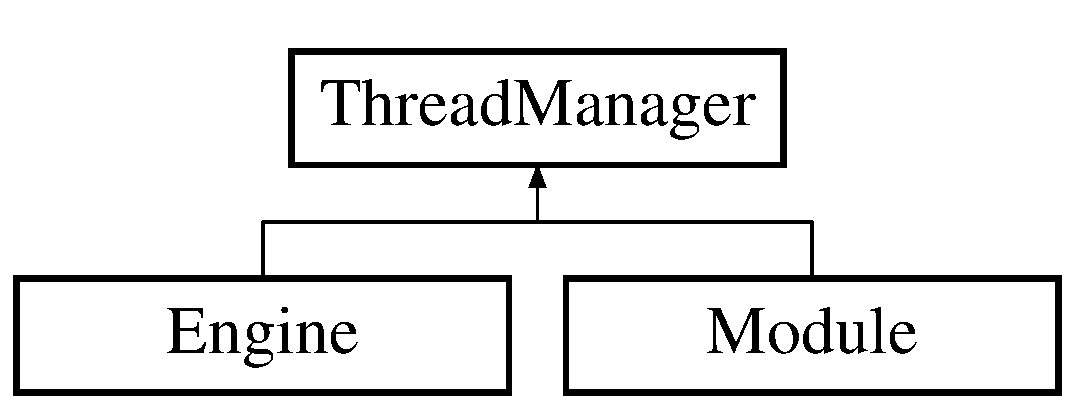
\includegraphics[height=2cm]{de/d57/classThreadManager}
\end{center}
\end{figure}
\subsection*{Public Member Functions}
\begin{DoxyCompactItemize}
\item 
virtual void \hyperlink{classThreadManager_afad6766592d98c6c0a2129f45e6a346e}{Create} (boost::shared\_\-ptr$<$ Thread $>$ thread)=0
\item 
virtual void \hyperlink{classThreadManager_a3c1b72b44ca4ffa3652088d44937b9d0}{Join} (int index)=0
\item 
\hypertarget{classThreadManager_abf5f1ccc763d5ecb13a8043552120741}{
virtual void {\bfseries Destroy} ()=0}
\label{de/d57/classThreadManager_abf5f1ccc763d5ecb13a8043552120741}

\item 
\hyperlink{classThreadManager_a613b13ebf45502e4d86c2f9317ec5871}{ThreadManager} ()
\item 
\hyperlink{classThreadManager_a18eb12d3d752075318c3672c8efffd5b}{$\sim$ThreadManager} ()
\end{DoxyCompactItemize}


\subsection{Constructor \& Destructor Documentation}
\hypertarget{classThreadManager_a613b13ebf45502e4d86c2f9317ec5871}{
\index{ThreadManager@{ThreadManager}!ThreadManager@{ThreadManager}}
\index{ThreadManager@{ThreadManager}!ThreadManager@{ThreadManager}}
\subsubsection[{ThreadManager}]{\setlength{\rightskip}{0pt plus 5cm}ThreadManager::ThreadManager ()}}
\label{de/d57/classThreadManager_a613b13ebf45502e4d86c2f9317ec5871}
default constructor \hypertarget{classThreadManager_a18eb12d3d752075318c3672c8efffd5b}{
\index{ThreadManager@{ThreadManager}!$\sim$ThreadManager@{$\sim$ThreadManager}}
\index{$\sim$ThreadManager@{$\sim$ThreadManager}!ThreadManager@{ThreadManager}}
\subsubsection[{$\sim$ThreadManager}]{\setlength{\rightskip}{0pt plus 5cm}ThreadManager::$\sim$ThreadManager ()}}
\label{de/d57/classThreadManager_a18eb12d3d752075318c3672c8efffd5b}
Destructor 

\subsection{Member Function Documentation}
\hypertarget{classThreadManager_afad6766592d98c6c0a2129f45e6a346e}{
\index{ThreadManager@{ThreadManager}!Create@{Create}}
\index{Create@{Create}!ThreadManager@{ThreadManager}}
\subsubsection[{Create}]{\setlength{\rightskip}{0pt plus 5cm}virtual void ThreadManager::Create (boost::shared\_\-ptr$<$ Thread $>$ {\em thread})\hspace{0.3cm}{\ttfamily  \mbox{[}pure virtual\mbox{]}}}}
\label{de/d57/classThreadManager_afad6766592d98c6c0a2129f45e6a346e}

\begin{DoxyParams}{Parameters}
\item[{\em thread}]\end{DoxyParams}


Implemented in \hyperlink{classEngine_a5de6694a069170d2205599331e6e8691}{Engine}, and \hyperlink{classModule_a9984bf9d8b1ea6e280c8c47cdb56e906}{Module}.

\hypertarget{classThreadManager_a3c1b72b44ca4ffa3652088d44937b9d0}{
\index{ThreadManager@{ThreadManager}!Join@{Join}}
\index{Join@{Join}!ThreadManager@{ThreadManager}}
\subsubsection[{Join}]{\setlength{\rightskip}{0pt plus 5cm}virtual void ThreadManager::Join (int {\em index})\hspace{0.3cm}{\ttfamily  \mbox{[}pure virtual\mbox{]}}}}
\label{de/d57/classThreadManager_a3c1b72b44ca4ffa3652088d44937b9d0}

\begin{DoxyParams}{Parameters}
\item[{\em index}]\end{DoxyParams}


Implemented in \hyperlink{classEngine_afe5c1c859cfe9b121627156dfbd58e6b}{Engine}, and \hyperlink{classModule_ac141815618543512136b7f4e0c90d311}{Module}.



The documentation for this class was generated from the following file:\begin{DoxyCompactItemize}
\item 
src/core/threadManager.h\end{DoxyCompactItemize}

\printindex
\end{document}
